%!TEX root = ../dokumentation.tex

\chapter{Routes}
\label{ch:Routes}
Die Routes beschreiben die URL-Pfade eines Servers die eine Anwendung aufrufen kann um eine Anfrage zu starten.
Der erste Einstiegspunkt der vorliegenden Anwendung ist - wie in der package.json beschrieben - die index.js Datei.

\begin{figure}[h]
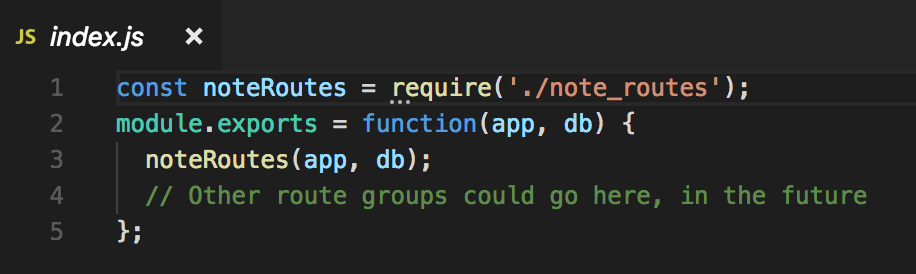
\includegraphics[height=.3\textwidth]{Serverindex.png}
\vspace{3pt}
\caption{index.js der Routes}
\label{fig:index.js der Routes}
\end{figure}

Wie in der ersten Zeile des Codesnippets (vgl. \autoref{fig:index.js der Routes}) beschrieben, importiert diese Datei eine weitere Datei namens \glqq note\_routes.js\grqq{}. Diese beinhaltet weitere Pfade die weitere \acs{API}'s zur Verfügung stellt.

\begin{figure}[h]
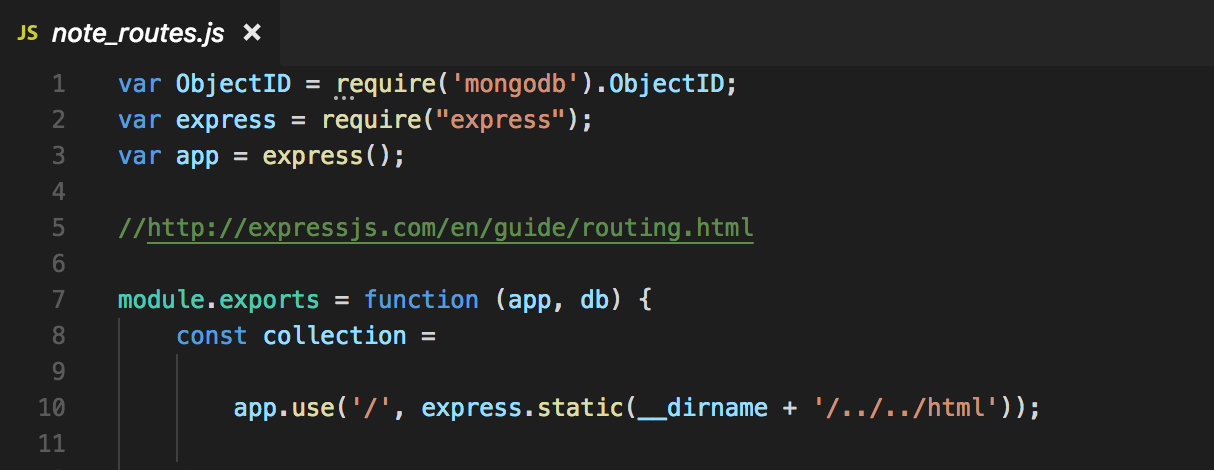
\includegraphics[height=.4\textwidth]{Routesmain.png}
\vspace{3pt}
\caption{Route-Imports}
\label{fig:Route-Imports}
\end{figure}

Die \glqq note\_routes.js\grqq -Datei beinhaltet die grundlegenden Verbindungen zur Mongo-Datenbank und dem Express-Framework. Durch diese haben die Routes die Möglichkeit, Requests zu verarbeiten und mit der Datenbank zu interagieren.

Die erste Route beschreibt das Verhalten für einen Request an die URL \glqq /\grqq . Die darauf folgende Reaktion ist die Auslieferung der Dateien die sich im übergeordneten Ordner \glqq html \grqq{}(vgl. \autoref{fig:Ordnerstruktur}) befinden.

Die folgenden Routes stehen zur Verfügung.
\begin{center}
\begin{figure}[h!]
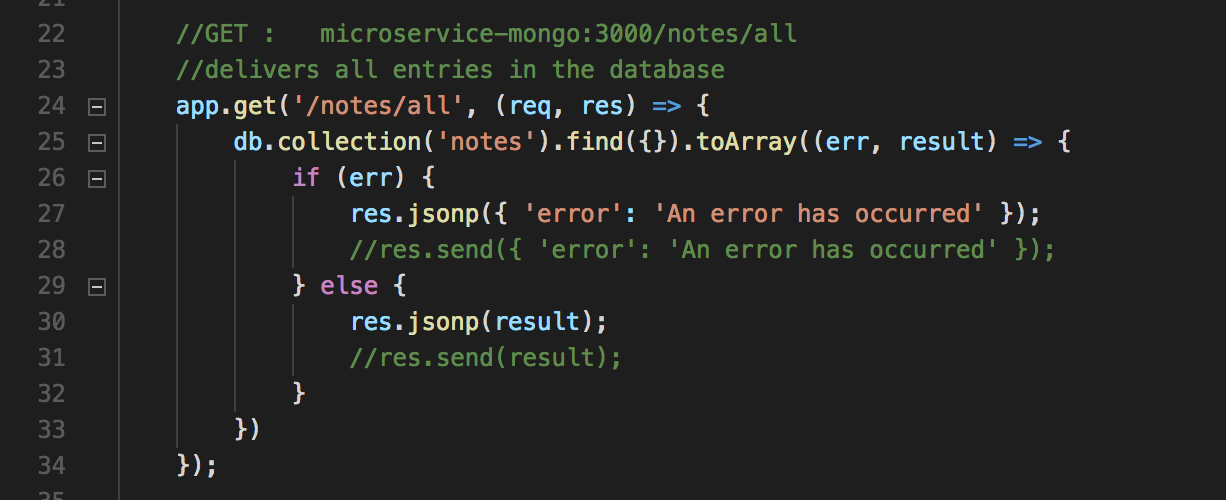
\includegraphics[height=.4\textwidth]{RoutesGetAll.png}
\vspace{1pt}
\caption{GetAll-Route}
\label{fig:GetAll-Route}
\end{figure}
\end{center}
Ein \textit{GET}-Request (vgl. \autoref{fig:GetAll-Route}) an die \glqq /notes/all\grqq{} liefert alle in der Datenbank verzeichneten Einträge als Response.
\begin{center}
\begin{figure}[h!]
\centering
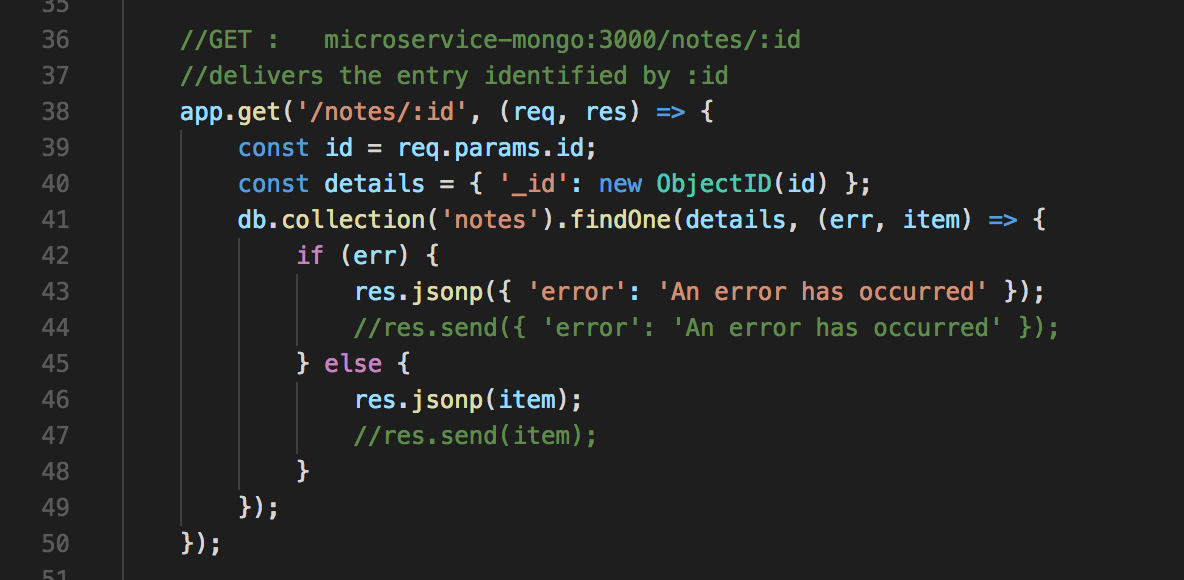
\includegraphics[height=.4\textwidth]{RoutesGetOne.png}
\vspace{1pt}
\caption{GetOne-Route}
\label{fig:GetOne-Route}
\end{figure}
\end{center}
Ein \textit{GET}-Request (vgl. \autoref{fig:GetOne-Route})  an die \glqq /notes/:id\grqq{} liefert den Eintrag der Datenbank mit der angegebenen ID als Response.

\begin{center}
\begin{figure}[h!]
\centering
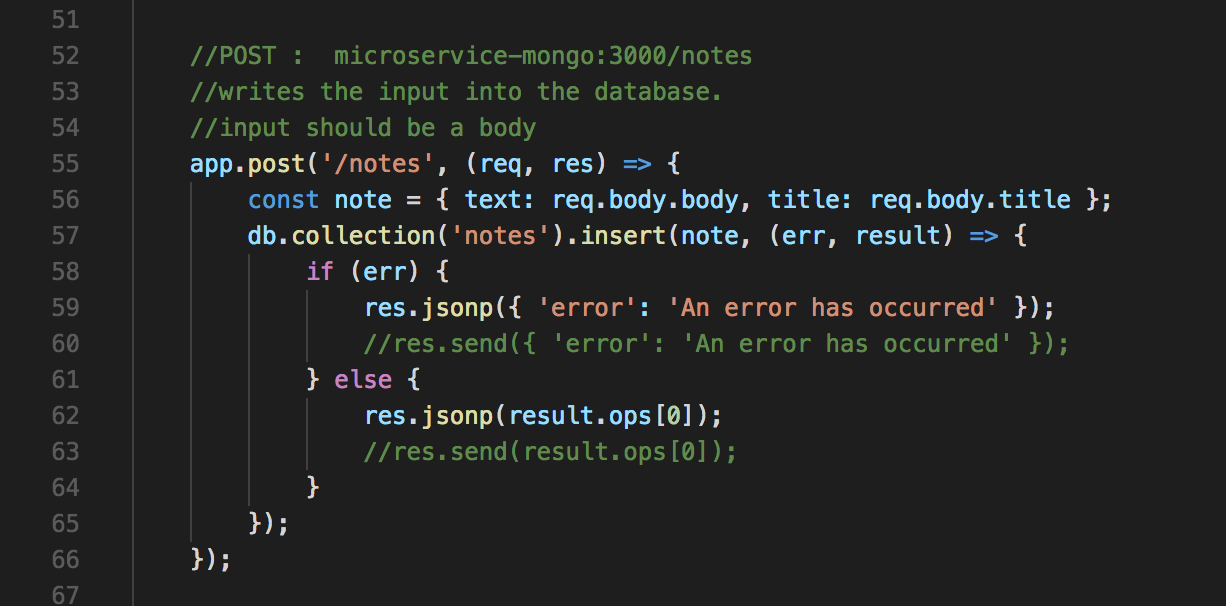
\includegraphics[height=.4\textwidth]{RoutesPost.png}
\vspace{1pt}
\caption{Post-Route}
\label{fig:Post-Route}
\end{figure}
\end{center}

Ein \textit{POST}-Request (vgl. \autoref{fig:Post-Route}) an die \glqq /notes\grqq{} schreibt den Inhalt des gesendeten Bodys in die Datenbank.

\begin{center}
\begin{figure}[h!]
\centering
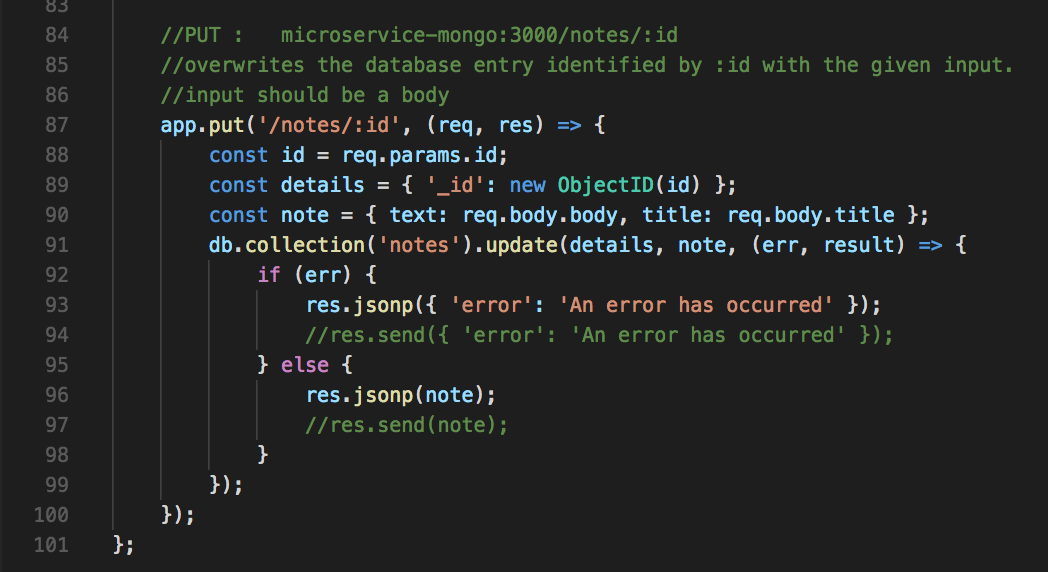
\includegraphics[height=.4\textwidth]{RoutesPut.png}
\vspace{1pt}
\caption{Put-Route}
\label{fig:Put-Route}
\end{figure}
\end{center}

Ein \textit{PUT}-Request (vgl. \autoref{fig:Put-Route}) an die \glqq /notes/:id\grqq{} ersetzt den Inhalt des Datenbankeintrags mit der angegebenen ID mit dem Body des Requests.

\begin{center}
\begin{figure}[H]
\centering
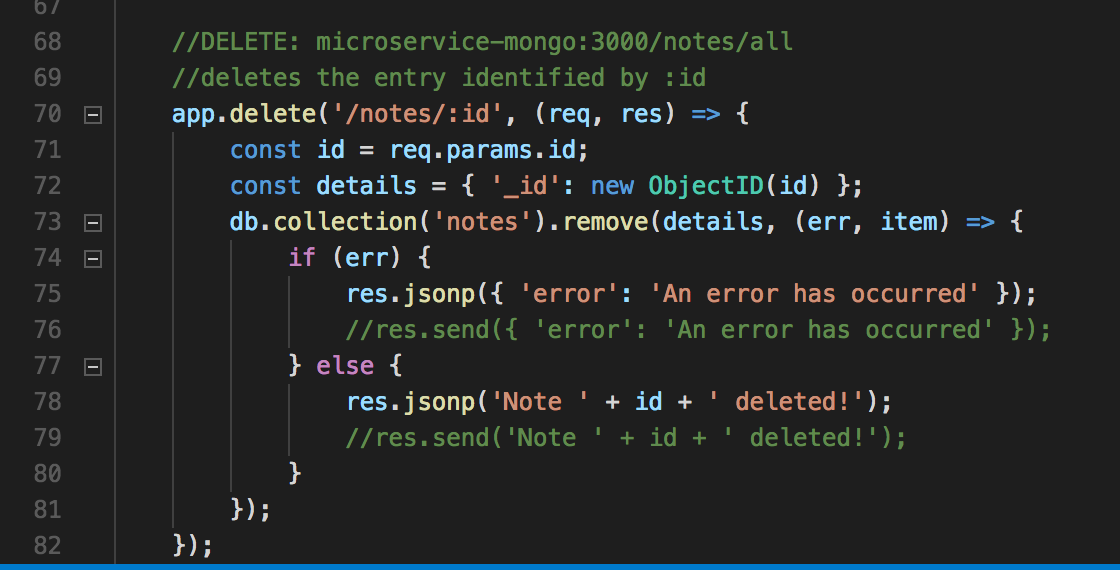
\includegraphics[height=.4\textwidth]{RoutesDelete.png}
\vspace{1pt}
\caption{Delete-Route}
\label{fig:Delete-Route}
\end{figure}
\end{center}
Ein \textit{DELETE}-Request (vgl. \autoref{fig:Delete-Route}) an die \glqq /notes/:id\grqq{} löscht den Datenbankeintrag mit der angegebenen ID.

